
\section{Evaluation}

We collected several data sets, however in this project due to page limit, only two of them that is collected in Soda Hall are shown in this section.

\label{sec:evaluation}

\subsection{Raw Data and Extracted Features: EDA}

The raw data sets are shown in figure (\ref{fig:soda1}) and (\ref{fig:soda2}) with ground truth labels. A quick glance tell us that the three devices we are using generate measurement of different quality as far as classification is concerned. For example, in all axis $\{x,y,z\}$, android phone yields measurement with little noise. 
\begin{figure*}
  \centering
  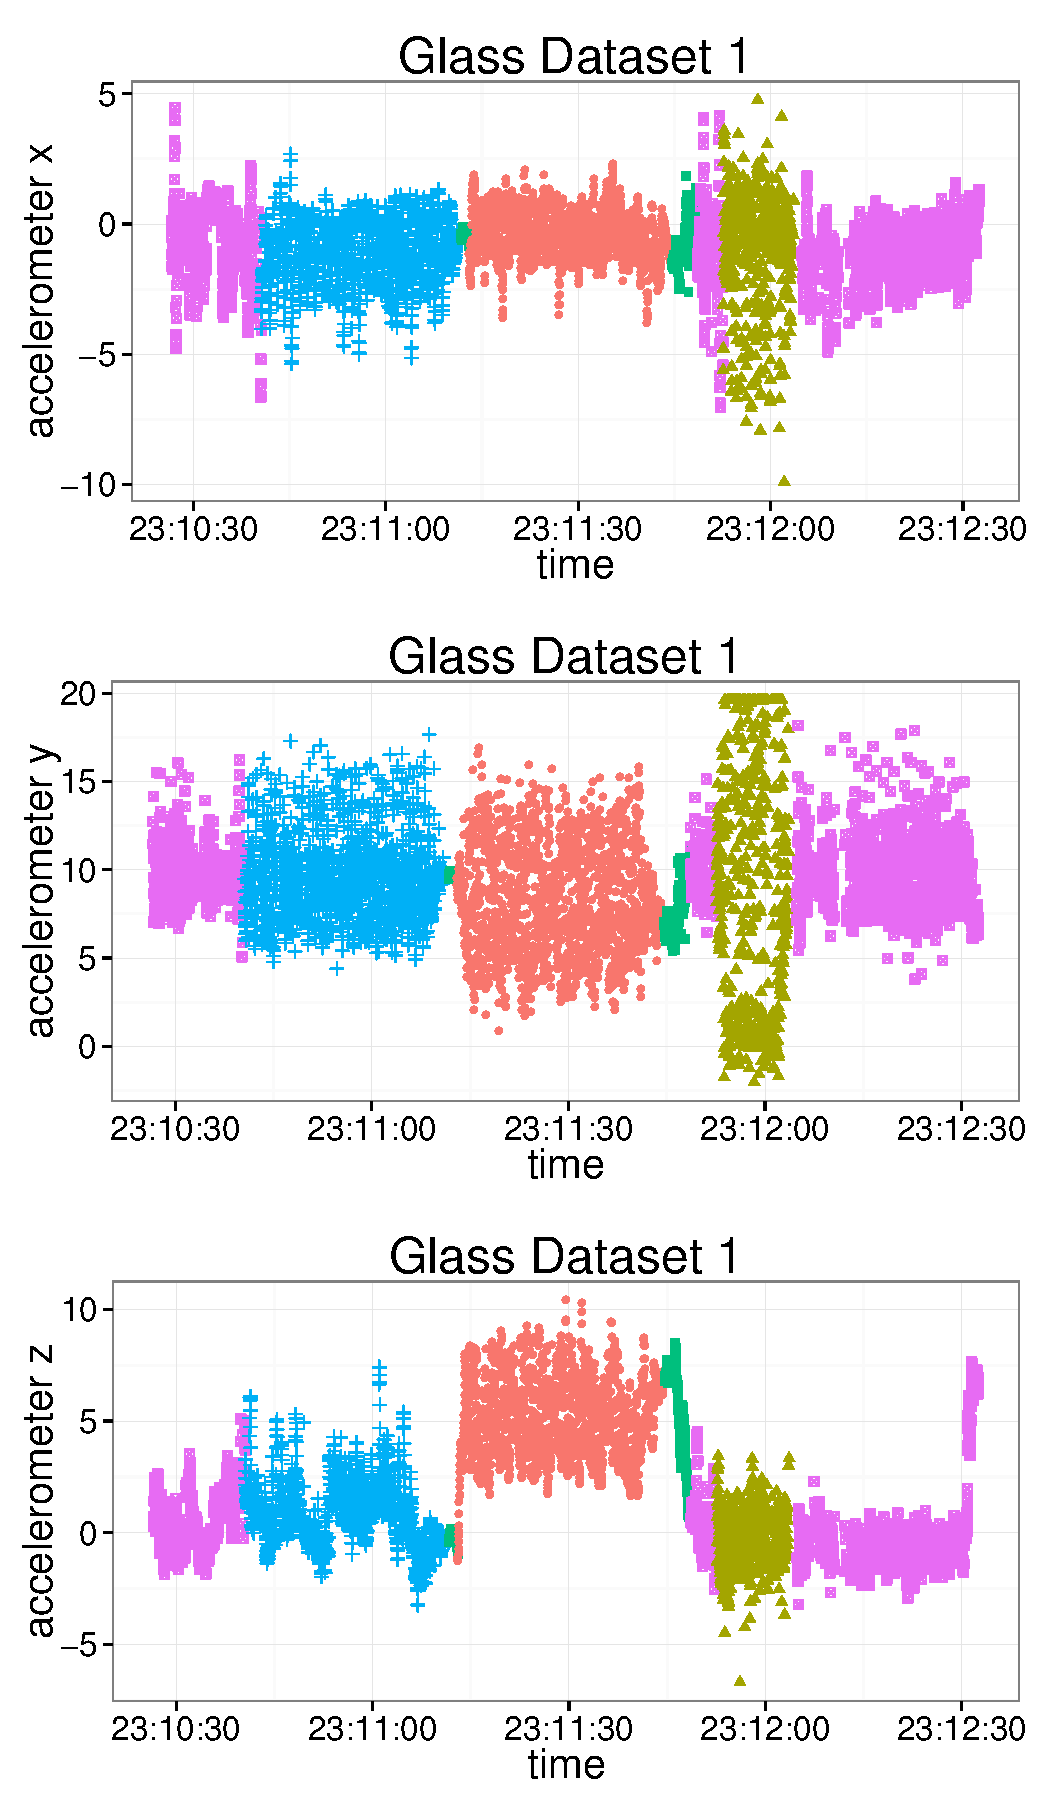
\includegraphics[width=0.3\textwidth]{figures/eda_soda1_glass.pdf}
  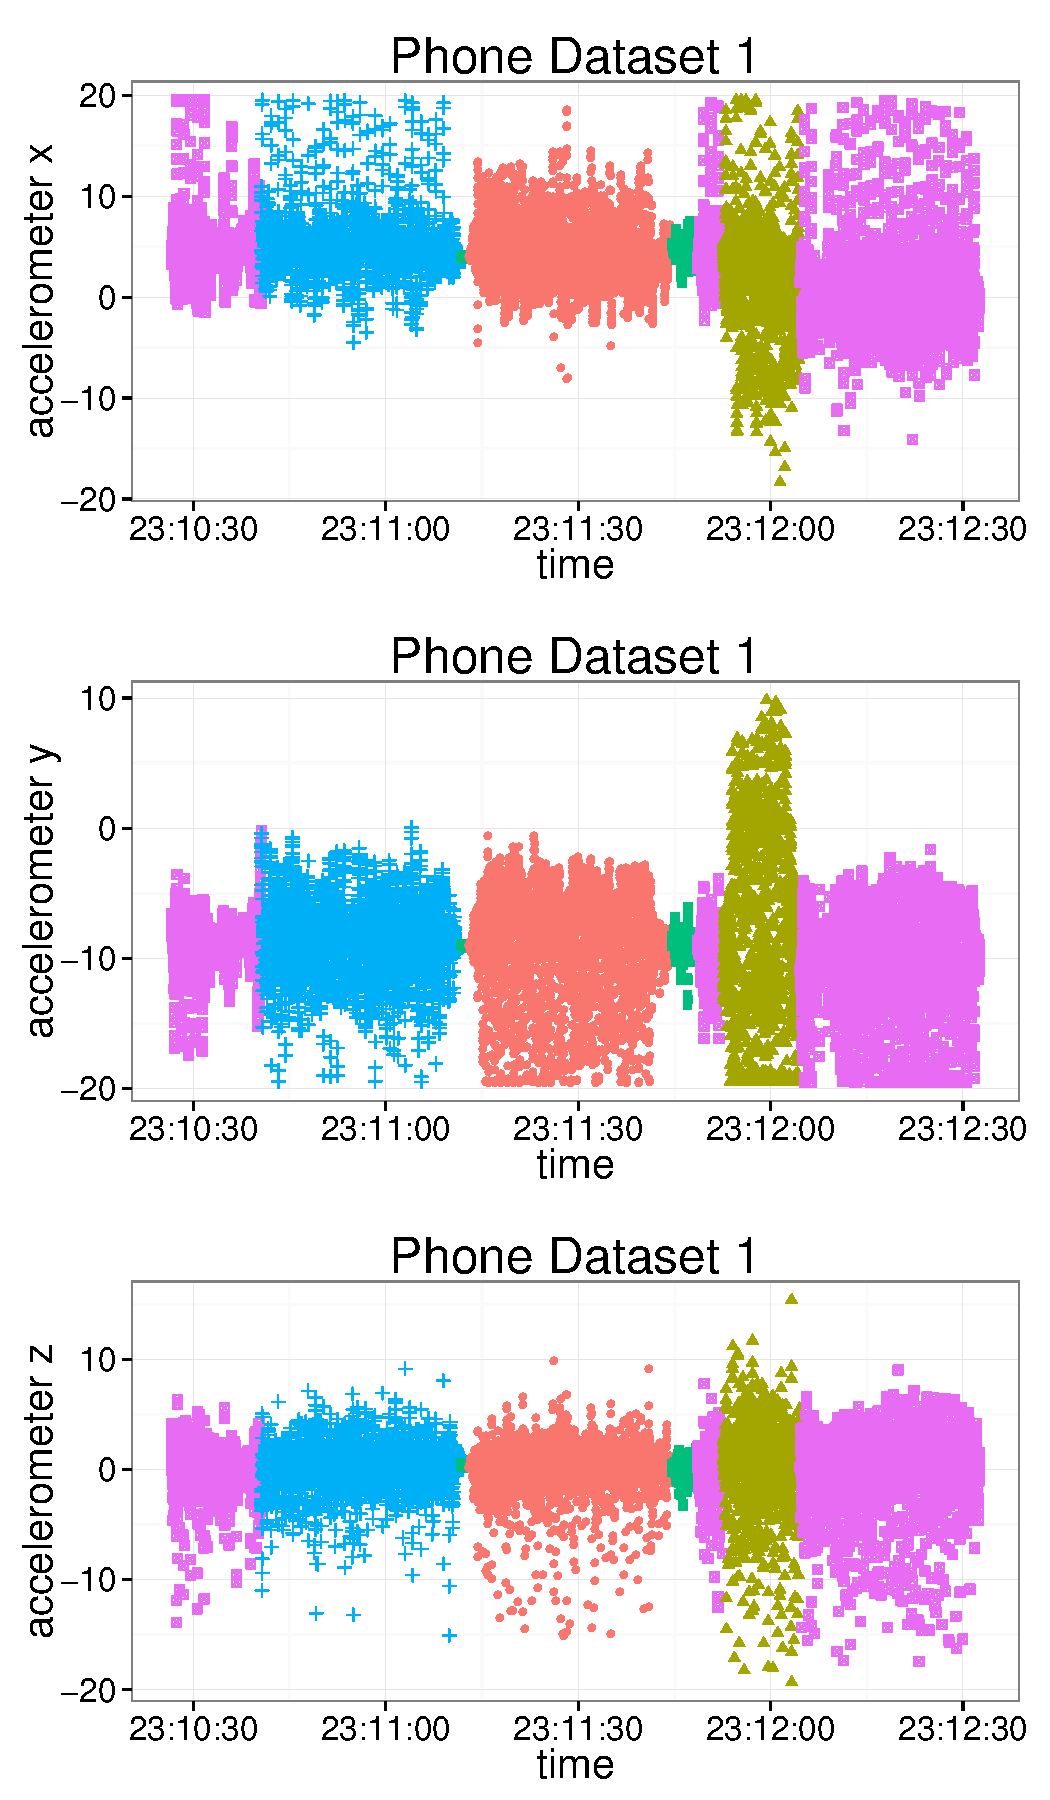
\includegraphics[width=0.3\textwidth]{figures/eda_soda1_phone.pdf}
  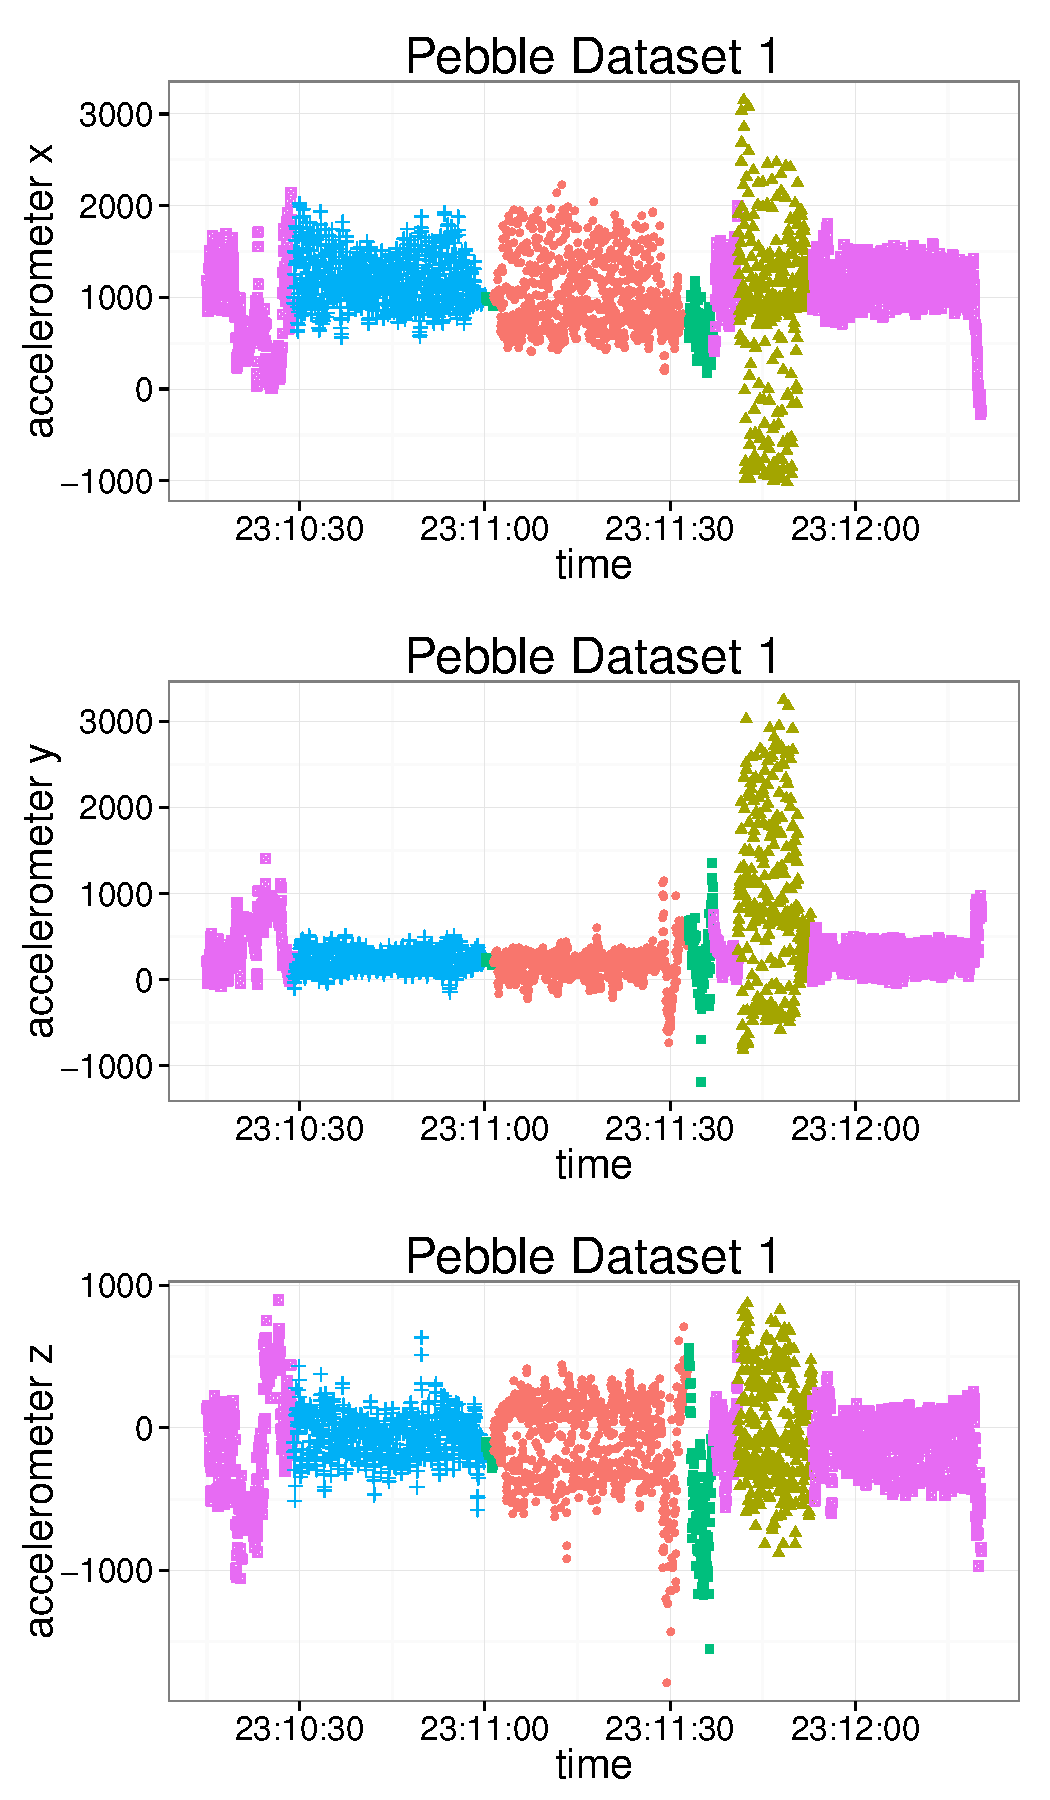
\includegraphics[width=0.3\textwidth]{figures/eda_soda1_pebble.pdf}
  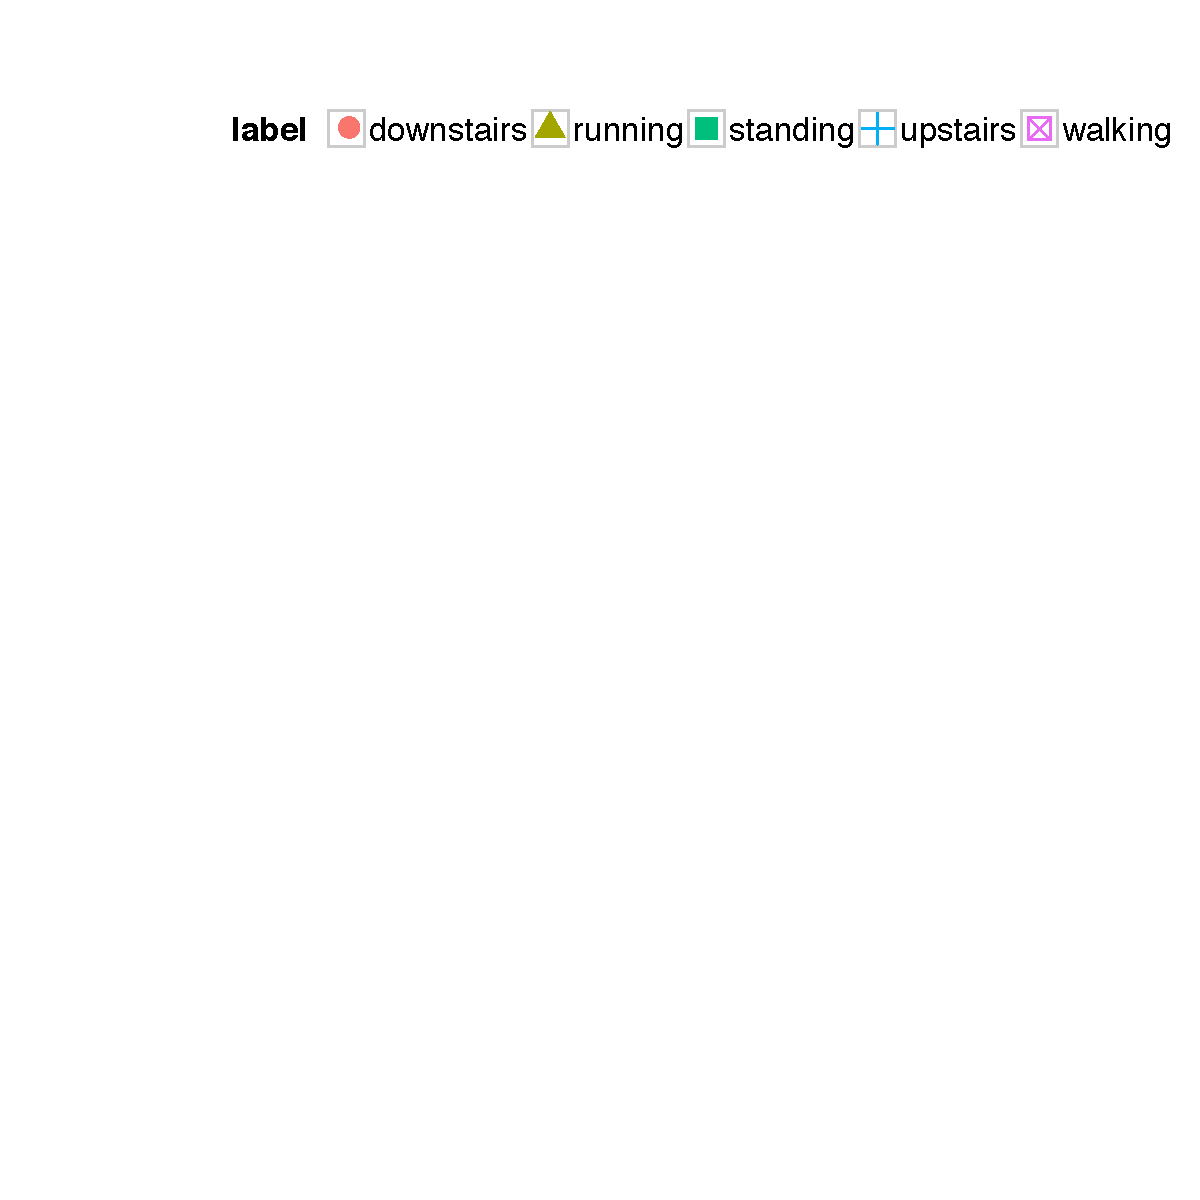
\includegraphics[width=0.5\textwidth]{figures/legend.pdf}
  \caption{The first raw data set visualization with groundtruth labeled.}
  \label{fig:soda1}
\end{figure*}

\begin{figure*}
  \centering
  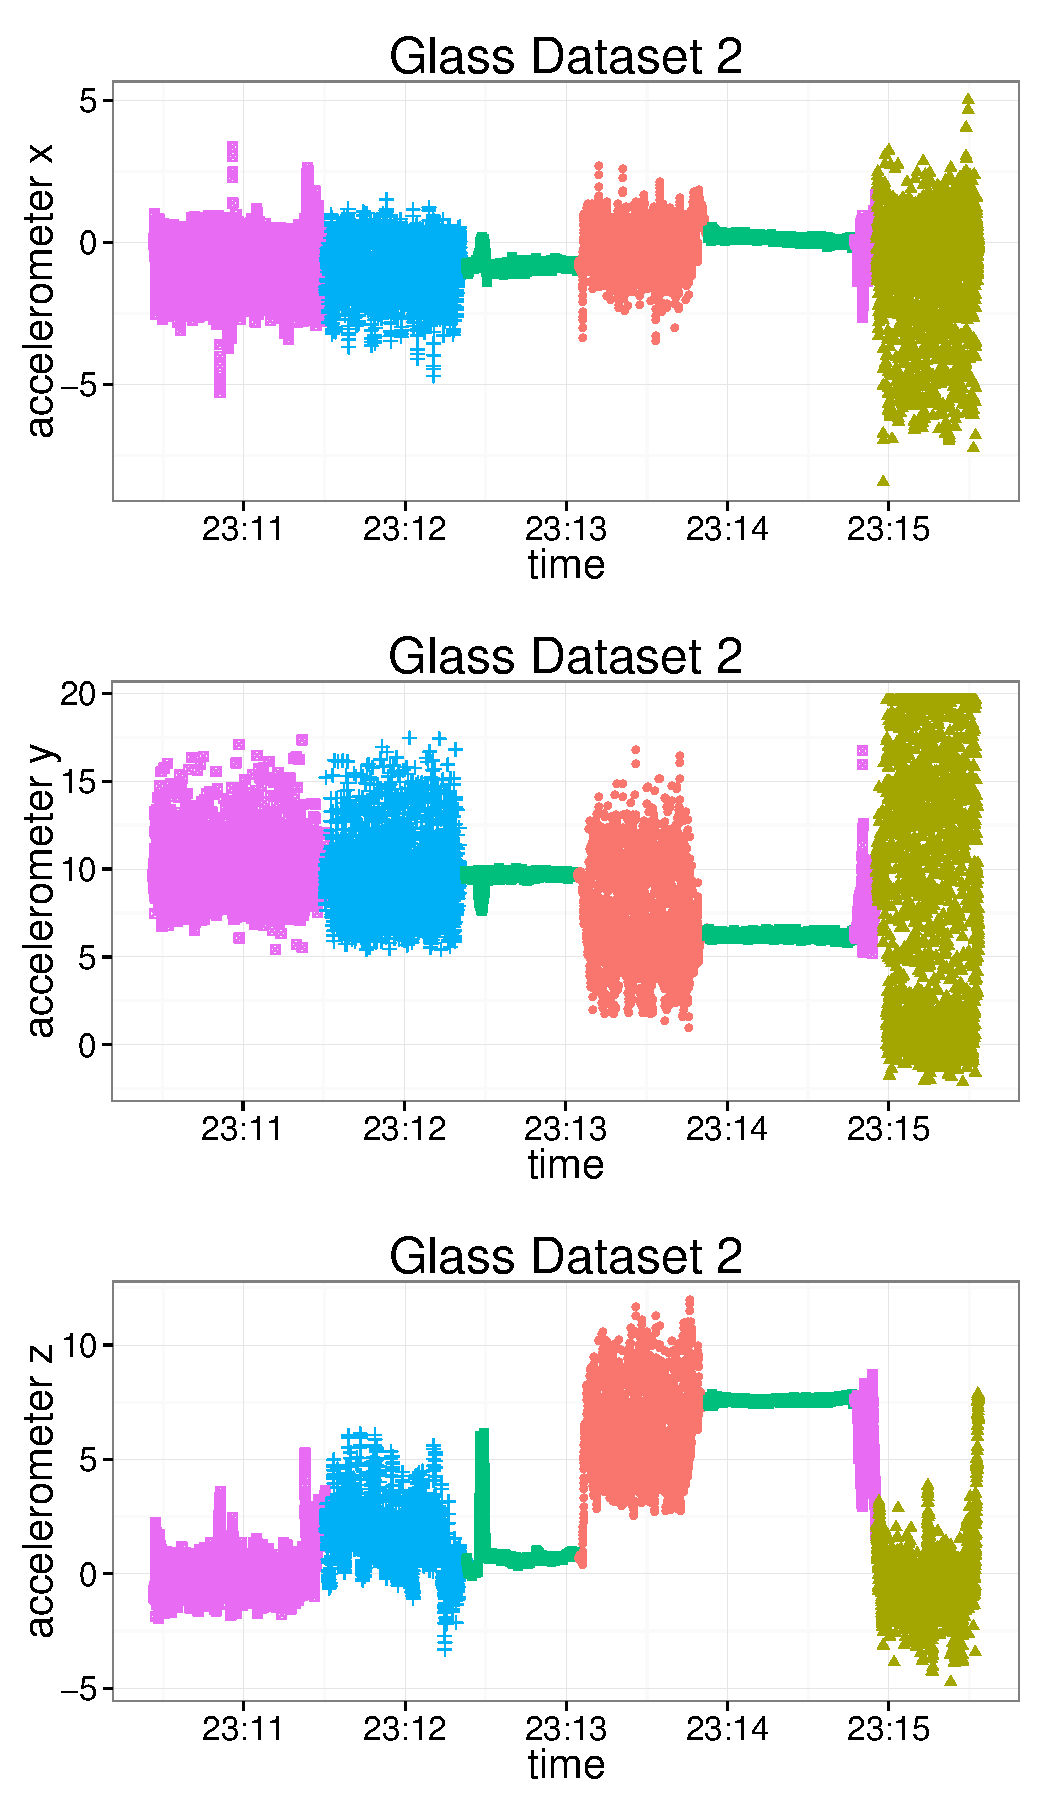
\includegraphics[width=0.3\textwidth]{figures/eda_soda2_glass.pdf}
  \includegraphics[width=0.3\textwidth]{figures/eda_soda2_phone.pdf}
  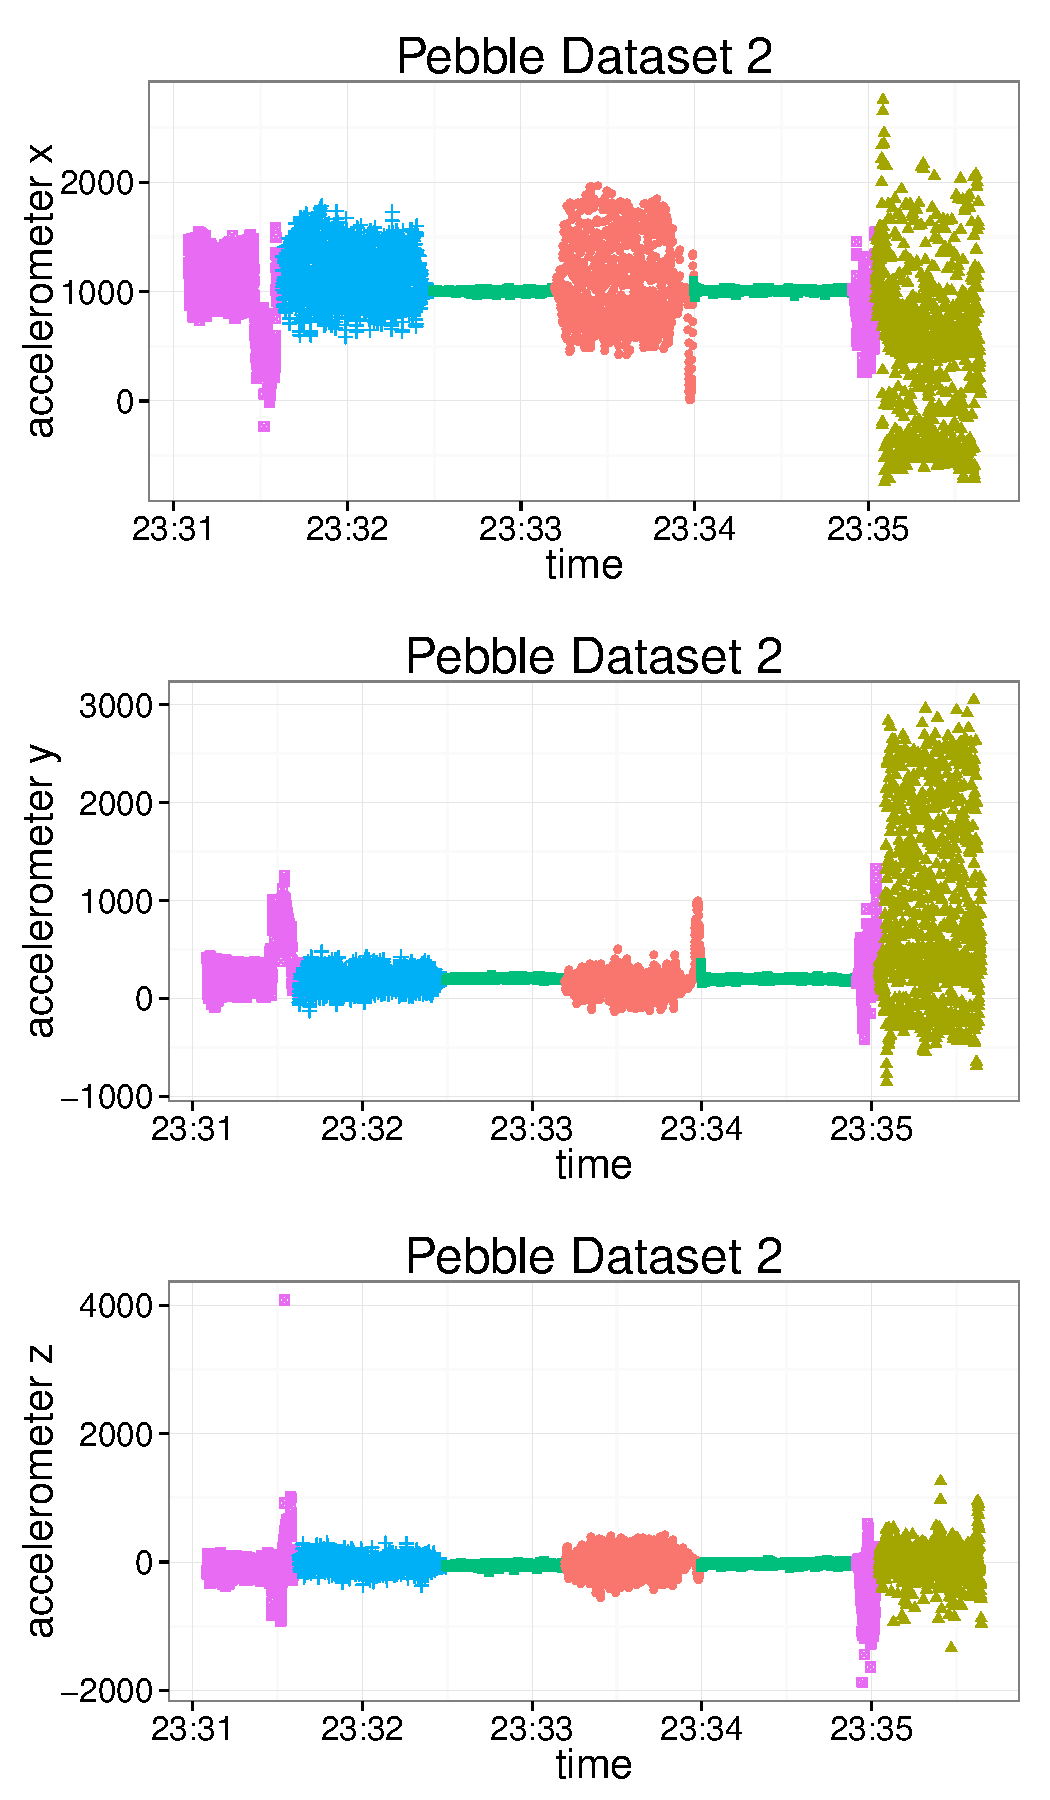
\includegraphics[width=0.3\textwidth]{figures/eda_soda2_pebble.pdf}
  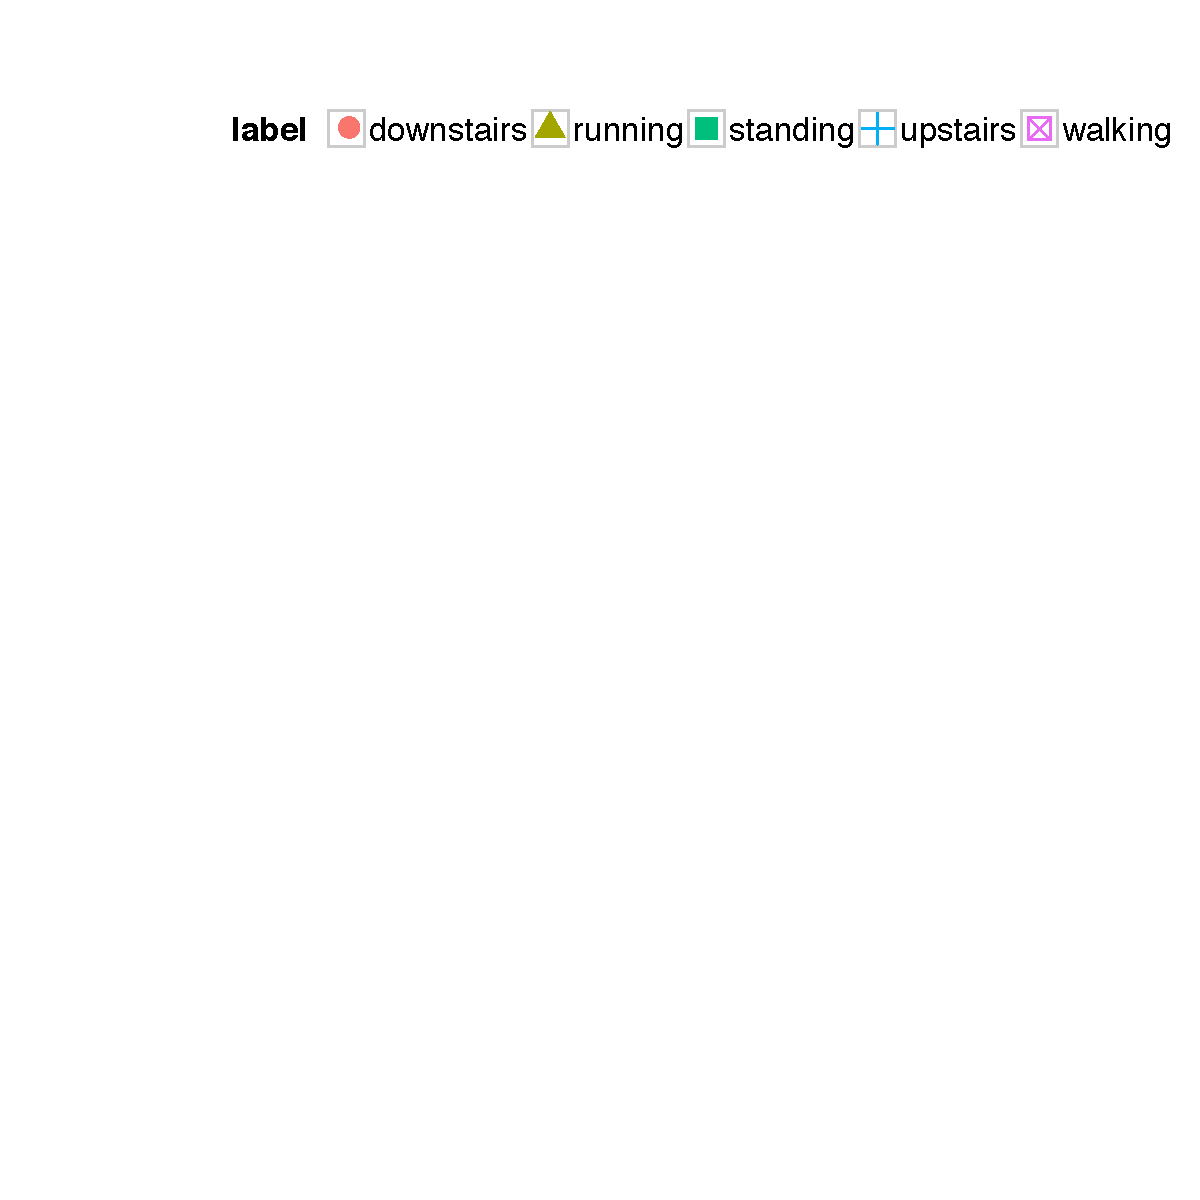
\includegraphics[width=0.5\textwidth]{figures/legend.pdf}
  \caption{The second raw data set visualization with groundtruth labeled.}
  \label{fig:soda2}
\end{figure*}

The empirical distribution for some selected features are shown in figure (\ref{fig:features}). We choose proper family of distribution for our HMM model by inspecting these empirical distributions, for example, we chose $Gamma$ distribution for Entropy,and multivariate Gaussian for $\bar{x},\bar{y},\bar{z}$. 

\begin{figure}[h]
  \centering
  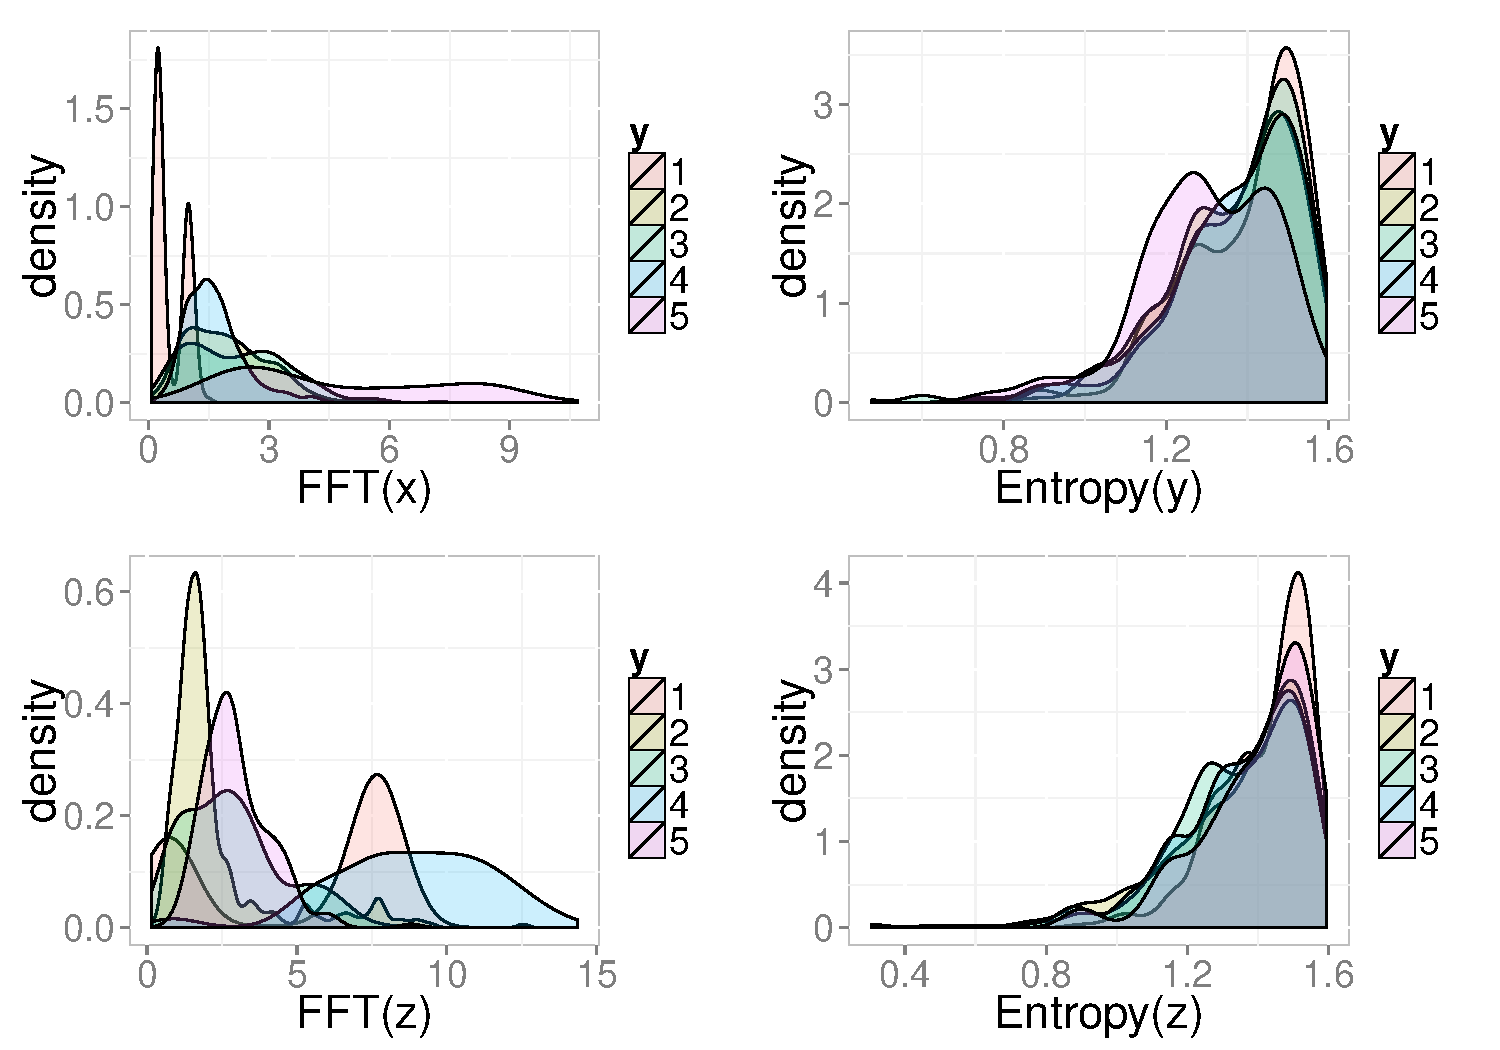
\includegraphics[width=0.45\textwidth]{figures/edafeature2.pdf}
  \caption{Empirical distribution for some selected features}
  \label{fig:features}
\end{figure}

In order to check the relation among features, we look at the pairwise scatter plot, and one  example of these plots containing frequency domain feature is shown in figure (\ref{fig:pairwise}). From this figure we can further justify the conditional dependence and independence of the features for HMM. For example, we use  multivariate Gaussian instead of 
single Gaussian for $\bar{x},\bar{y},\bar{z}$, since they exhibit a strong correlation when conditioning on a specific activity.
\begin{figure}[h]
  \centering
  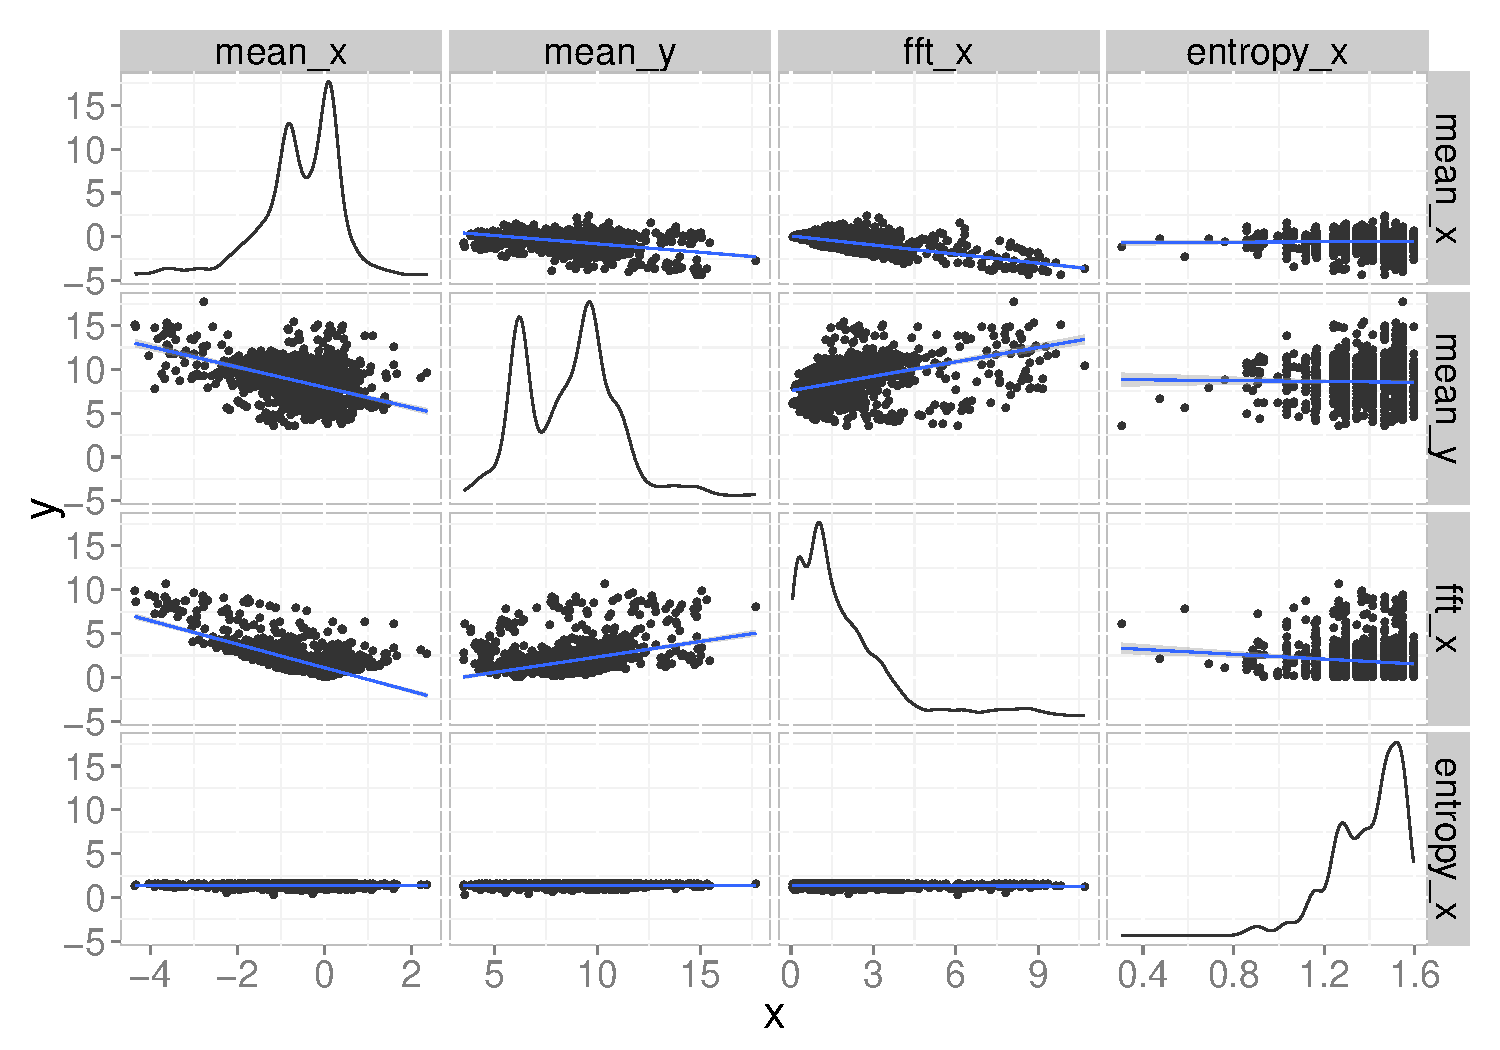
\includegraphics[width=0.45\textwidth]{figures/edafeature1.pdf}
  \caption{Pairwise scatter plot for some features}
  \label{fig:pairwise}
\end{figure}


\subsection{Classification Results}

Both model fitting and testing errors are summarized in terms of overall accuracy and cross error table to indicate the performance of activity recognition with three different devices and two different learning methods. Let's examine the results in a device order for easy comparison.

\subsubsection{Google Glass Results}
\label{sec:glassresult}
\begin{itemize}
\item \textbf{With Multinomial Logistic Regression} 
The results are shown in table (\ref{tab:glassLR1}) and (\ref{tab:glassLR2})

\begin{table}[h]
\begin{center}
\begin{tabular}{|l|l|}
      \hline
      Training Accuracy & Testing Accuracy\\
      \hline
      $0.9036635$ & $0.7469244$ \\
      \hline
\end{tabular}
\caption{Google Glass with LR: overall accuracy}
\label{tab:glassLR1}
\end{center}
\end{table}

\begin{table}[h]
\begin{center}
\begin{tabular}{|l|l|l|l|l|l|}
      \hline
      P/T& 1 & 2 &3 & 4 & 5 \\
      \hline
      1 &0.625&0.032&0.020&0.057&0.000\\
      2 &0.125&0.727&0.188&0.057&0.107\\
      3 &0.250&0.199&0.651&0.007&0.071\\
      4 &0.000&0.041&0.114&0.878&0.053\\
      5 & 0.000&0.000&0.026&0.000&0.767\\
      \hline
\end{tabular}
\caption{Google Glass with LR: Cross Error Table}
\label{tab:glassLR2}
\end{center}
\end{table}
\item \textbf{With HMM}
The results are shown in table (\ref{tab:glassHMM1}) and (\ref{tab:glassHMM2})

\begin{table}[h]
\begin{center}
\begin{tabular}{|l|l|}
      \hline
      Training Accuracy & Testing Accuracy\\
      \hline
      $0.9599729$ & $0.7188049$ \\
      \hline
\end{tabular}
\caption{Google Glass with HMM: overall accuracy}
\label{tab:glassHMM1}
\end{center}
\end{table}
\begin{table}[h]
\begin{center}
\begin{tabular}{|l|l|l|l|l|l|}
      \hline
      P/T& 1 & 2 &3 & 4 & 5 \\
      \hline
      1 &0.400&0.057&0.006&0.029&0.000\\
      2 &0.066&0.692&0.240&0.067&0.155\\
      3 &0.133&0.211&0.629&0.022&0.017\\
      4 &0.400&0.033&0.110&0.880&0.068\\
      5 & 0.000&0.005&0.013&0.000&0.759\\
      \hline
\end{tabular}
\caption{Google Glass with HMM: Cross Error Table}
\label{tab:glassHMM2}
\end{center}
\end{table}
\end{itemize}

As expected, the testing error is much higher than training error for both Logistic Regression and HMM, while on testing set our system and algorithm still gives above 70\% accuracy. 

More interesting results can be revealed by looking at cross error table. Note that the number $\{1,2,...,5\}$ represent \{standing, walking, downstairs, upstairs, running\}. The rows of the table are ground truth and the columns are predicted value, thus the $\{i,j\}^{th}$ element of the table is interpreted as \textit{predicted value is $i$, while the true value should be $j$}. From this interpretation we see the diagonal terms in the table are actually accuracy in each class, and cross terms are different classification errors. \footnote{We normalize the error in each class, however different classes may have different sample size.}

We observe that in the case of using Google glass, the logistic regression method performs a little better than with HMM. Specifically, in both algorithms, Google glass distinguished very well the \textit{upstairs} state. Intuitively, this could be explained by the fact that when people are going upstairs, their head usually look up and maintains a distinct position, while in other states, people tend to move their head occasionally, which produce additional noise to Google glass measurement and harms the classification. This phenomena can also been seen especially from the fact that, for Google glass data with both algorithm, the standing state yields the most error.

Note also that we did not see improvement by incorporating transition (by using HMM), however, it does not exclude the benefit of transitional information. Actually, since our data set only measures a relatively short period, and the transitions of states are not statistically sufficient, we assume that for longer data with more complicated transitions, HMM method should show its advantages. 

\subsubsection{Android Phone Results} 
\label{subsec:phoneresult}
\begin{itemize}

\item \textbf{With Multinomial Logistic Regression} 
The results are shown in table (\ref{tab:phoneLR1}) and (\ref{tab:phoneLR2})

\begin{table}[h]
\begin{center}
\begin{tabular}{|l|l|}
      \hline
      Training Accuracy & Testing Accuracy\\
      \hline
      $0.748297$ & $0.3341772$ \\
      \hline
\end{tabular}
\caption{Phone with LR: overall accuracy}
\label{tab:phoneLR1}
\end{center}
\end{table}

\begin{table}[h]
\begin{center}
\begin{tabular}{|l|l|l|l|l|l|}
      \hline
      P/T& 1 & 2 &3 & 4 & 5 \\
      \hline
      1 &0.593&0.125&0.071&0.017&0.000\\
      2 &0.196&0.125&0.313&0.366&0.318\\
      3 &0.125&0.000&0.306&0.241&0.181\\
      4 &0.129&0.125&0.282&0.294&0.272\\
      5 &0.062&0.625&0.026&0.080&0.227\\
      \hline
\end{tabular}
\caption{Phone with LR: Cross Error Table}
\label{tab:phoneLR2}
\end{center}
\end{table}

\item \textbf{With HMM}
The results are shown in table (\ref{tab:phoneHMM1})and (\ref{tab:phoneHMM2})

\begin{table}[h]
\begin{center}
\begin{tabular}{|l|l|}
      \hline
      Training Error & Testing Error\\
      \hline
      $0.9591281$ & $0.3578059$ \\
      \hline
\end{tabular}
\caption{Phone with HMM: overall accuracy}
\label{tab:phoneHMM1}
\end{center}
\end{table}
\begin{table}[h]
\begin{center}
\begin{tabular}{|l|l|l|l|l|l|}
      \hline
      P/T& 1 & 2 &3 & 4 & 5 \\
      \hline
      1 &1&0.014&0.064&0.006&0.000\\
      2 &0&0.542&0.303&0.635&0.158\\
      3 &0&0.136&0.335&0.155&0.123\\
      4 &0&0.188&0.271&0.162&0.341\\
      5 & 0&0.117&0.026&0.040&0.376\\
      \hline
\end{tabular}
\caption{Phone with HMM: Cross Error Table}
\label{tab:phoneHMM2}
\end{center}
\end{table}
\end{itemize}

We observe that both algorithm performed terribly on Android phone data set. In effect, from previous part of EDA we already have a sense that phone data set is more noisy and indistinguishable. The reason for that is simple: we put the android phone in the trousers pocket, and in all states except for standing, people's legs move periodically with a similar pattern. Hence we see that with phone data set only the standing state is well classified, even with 1 accuracy with HMM, other states are mixed together and both classifiers only performs slightly better than a random guess. 

\subsubsection{Pebble Watch Results}
\label{subsec:pebbleresult}
\begin{itemize}
\item \textbf{With Multinomial Logistic Regression} 
The results are shown in table (\ref{tab:pebbleLR1}) and (\ref{tab:pebbleLR2})

\begin{table}[h]
\begin{center}
\begin{tabular}{|l|l|}
      \hline
      Training Accuracy & Testing Accuracy\\
      \hline
      $0.8658537$ & $0.6677966$ \\
      \hline
\end{tabular}
\caption{Pebble with LR: overall accuracy}
\label{tab:pebbleLR1}
\end{center}
\end{table}

\begin{table}[h]
\begin{center}
\begin{tabular}{|l|l|l|l|l|l|}
      \hline
      P/T& 1 & 2 &3 & 4 & 5 \\
      \hline
      1 &0.166&0.065&0.000&0.013&0.000\\
      2 &0.166&0.631&0.274&0.083&0.242\\
      3 &0.000&0.163&0.709&0.111&0.060\\
      4 &0.166&0.131&0.000&0.763&0.090\\
      5 &0.500&0.0082&0.016&0.027&0.606\\
      \hline
\end{tabular}
\caption{Pebble with LR: Cross Error Table}
\label{tab:pebbleLR2}
\end{center}
\end{table}

\item \textbf{With HMM}
The results are shown in table (\ref{tab:pebbleHMM1})and (\ref{tab:pebbleHMM2})

\begin{table}[h]
\begin{center}
\begin{tabular}{|l|l|}
      \hline
      Training Accuracy & Testing Accuracy\\
      \hline
      $0.9318902$ & $ 0.6237288$ \\
      \hline
\end{tabular}
\caption{Pebble with HMM: overall accuracy}
\label{tab:pebbleHMM1}
\end{center}
\end{table}
\begin{table}[h]
\begin{center}
\begin{tabular}{|l|l|l|l|l|l|}
      \hline
      P/T& 1 & 2 &3 & 4 & 5 \\
      \hline
      1 &0.5&0.063&0.000&0.019&0.000\\
      2 &0.0&0.618&0.370&0.182&0.080\\
      3 &0.5&0.218&0.555&0.183&0.000\\
      4 &0.0&0.081&0.074&0.596&0.000\\
      5 &0.0&0.018&0.000&0.019&0.920\\
      \hline
\end{tabular}
\caption{Pebble with HMM: Cross Error Table}
\label{tab:pebbleHMM2}
\end{center}
\end{table}
\end{itemize}

The results for Pebble data could be analyzed similarly. The performance of our classifier on this data set is in the middle of the performance on last two data sets. One interesting phenomenon is that the running state is very well classified, which could also be explained by intuition. When people are running, their forearm usually move with much higher frequency than in any other states. The classification of running versus other activities are relatively simple because in our feature selection procedure, we also include frequency domain features. 

To sum up, we have observed that measurements of different devices can help to distinguish different activities. As is mentioned above, this specialization comes from the fact that three devices are actually measuring the movement of different parts of human body. Therefore we propose that a combined sensoring system could greatly improve the classification performance of activity recognition. Major part of our future work will be devoted to this direction. 

%%% Local Variables: 
%%% mode: latex
%%% TeX-master: "main"
%%% End: 
